
\section{상세 분석}

\subsection{최악의 케이스 분석 }


실제 재귀함수를 일반화 식은 다음이 된다.

$$T(n) = \max_{0 \le q \le n-1}(T(q) + T(n-q-1)) + \Theta(n)$$

이때 $T(n)$이 $\Theta(n^2)$임을 보이면된다.
치환법을 이용해서 이 점화식을 풀수있다.
$T(n) \le c_1n^2$이라 가정하자. 그러면

$$T(n) \le \max_{0 \le q \le n-1}(c_1q^2 + c_1(n-q-1)^2) + \Theta(n)$$

이 성립한다. 

$0 \le q \le n-1$인 $c_1q^2 + c_1(n-q-1)^2$에 대해서 

$f(q) = c_1q^2 + c_1(n-q-1)^2$ 이라하고 $f'(q) = 2c_1q - 2c_1(n-q-1)$이므로 $q=\dfrac{n-1}{2}$일때 극솟값을 가진다. 이 극솟값은 $q$의 존재 범위에 포함되고 따라서 이차함수의 특성에 따라 양 끝점이 최댓값이 될수있는 후보가된다. $q=0$일때와 $q=n-1$일때 극댓값을 가지는데 이때의 두 함숫값은 같아서 둘중 어느값을 택해도 최댓값이 된다.

\begin{align*}
    T(n) & \le c_1(n-1)^2 + \Theta(n) \\
    & \le c_1n^2 - c(2n-1) + \Theta(n) \\
    & \le c_1n^2    
\end{align*}


이때 $\Theta(n) = dn$에서 $ c_1 > d $인 상수 $c_1$을 가지게 함으로 써 결과적으로 $T(n)$이 $c_1n^2$보다 작거나 같음을 보일수있다. 반대로 $c_2n^2 \le T(n)$임을 가정하고  $ c_2 < d $인 상수를 잡음으로 $T(n)$이 $c_2n^2$보다 크거나 같음을 보일수있다. 따라서 $T(n) = \Theta(n^2)$를 얻을 수 있다.


\subsection{기대 수행 시간}

1 부터 모든 n에 대해서 모든 비용의 평균.

%$\dfrac{\sum_{i=1}^{n}E[X_i]}{n}$

\begin{align*}
    E[X] &= E\left[ \sum_{i=1}^{n}X_i \right] \\
    &= \sum_{i=1}^{n}E\left[X_i \right]   
\end{align*}
 
시간복잡도를 분석하기위해서 다음의 보조정리를 이용한다.


% Let X be the number of comparisons performed in line 4 of PARTITION over the entire execution of QUICKSORT on an n-element array. 

% Then the running time of QUICKSORT is O(n + X)
\begin{lemma}
    X가 길이가 n인 배열에서 QUICKSORT의 전체 실행에 대해서 PARTITION의 4행에서 수행된 비교문의 실행 수라고 가정하면 QUICKSORT의 실행시간은 O(N+X)이다.    
\end{lemma}


% By the discussion above, the algorithm makes at most n calls to PARTITION, each of which does a constant amount of work and then executes the for loop some number of times. 
% Each iteration of the for loop executes line 4.

%  PARTITION에 대한 모든 호출에서 수행 된 비교의 총 수인 X를 계산하는 것이다.

% PARTITION에 대한 각 호출에서 얼마나 많은 비교가 이루어 졌는지 분석하려고 시도하지 않습니다.

%  오히려 총 비교 수에 대한 전반적인 경계를 유도합니다.

\begin{proof}
    알고리즘은 PARTITION을 최대 n 회 호출한다. 각 호출은 for 루프를 실행하는데, for 루프의 각 반복은 4행 비교문을 실행한다.    
\end{proof}

따라서 모든 호출에 대해서 총 비교수 X를 구하는 문제로 바뀌는데 각 호출에 대한 비교를 분석하지않고 총 비교수를 계산한다.
그렇게 하기 위해 배열 $A = \{z_1 , z_2, ... , z_n\}$의 각 요소가 내림차순으로 정렬되어있다고 생각한다. 또한 집합 $Z_{ij} = \{z_i, z_{i+1}, ..., z_j\}$라 정의한다. 여기서 $z_i$와 $z_j$는 최대 한번 비교된다. 이유는 PARTITION에서 비교를 하는 경우는 하나의 원소가 pivot으로 선택 되었을 때인데, 이후에 이 pivot은 절대로 다른 원소와 비교하지 않는다.
따라서
%indicator random variables
$X_{ij} = I\{ z_i$가 $z_j$와 비교한다 $\}$

$ X = \sum_{i=1}^{n-1}\sum_{j=i+1}^{n} X_{ij}$

\begin{align*}
    E[x] &= E \left[ \sum_{i=1}^{n-1}\sum_{j=i+1}^{n} X_{ij} \right] \\
    &= \sum_{i=1}^{n-1}\sum_{j=i+1}^{n} E\left[X_{ij} \right] \\
    &= \sum_{i=1}^{n-1}\sum_{j=i+1}^{n}Pr\{ z_i \mbox{가} z_j\mbox{와 비교한다} \} 
\end{align*}    
    
\begin{align*}
    Pr\{ z_i \mbox{가} z_j\mbox{와 비교한다} 
    &= Pr\{ Z_{ij}\mbox{에서} z_i \mbox{또는} z_j\mbox{가 첫번째로 선택된다.}\}\\
    &= Pr\{ Z_{ij} \mbox{에서} z_i \mbox{가 첫번째로 선택된다}.\} + Pr\{ Z_{ij}\mbox{에서} z_j \mbox{가 첫번째로 선택된다.}\} \\
    &= \dfrac{1}{j-i+1} + \dfrac{1}{j-i+1} \\
    &= \dfrac{2}{j-i+1}    
\end{align*}
    

$$E[X] =  \sum_{i=1}^{n-1}\sum_{j=i+1}^{n} \dfrac{2}{j-i+1}$$

이는 $j-i$을 $k$로 치환해서 상한을 얻을 수 있다.

\begin{align*}
    E[X] & = \sum_{i=1}^{n-1}\sum_{j=i+1}^{n} \dfrac{2}{j-i+1}\\
    & =  \sum_{i=1}^{n-1}\sum_{k = 1}^{n-i} \dfrac{2}{k+1} \\
    & \le \sum_{i=1}^{n-1}\sum_{k = 1}^{n} \dfrac{2}{k} \\
    & \le \sum_{i=1}^{n-1} c\lg n \\
    & \le c n \lg n    
\end{align*}


$$E[X]= O(n \lg n)$$

하한은 다음과 같이 직접구한다.
\begin{align*}    
E[X] &= \sum_{i=1}^{n-1}\sum_{k = 1}^{n-i} \dfrac{2}{k+1} \\
& = \sum_{k = 1}^{n-1} \dfrac{2}{k+1} + \sum_{k = 1}^{n-2} \dfrac{2}{k+1} + \cdots + \sum_{k = 1}^{1} \dfrac{2}{k+1}\\
& = (n-1)\dfrac{2}{1+1} + (n-2)\dfrac{2}{2+1} + \cdots +1 \times \dfrac{2}{(n-1)+1}\\
& = \sum_{k=1}^{n-1} \dfrac{2}{k+1} \times (n-k)\\
& = \sum_{k=1}^{n-1} \left( \dfrac{2n}{k+1} -\dfrac{2k}{k+1}\right)\\
& = 2n \sum_{k=1}^{n-1} \dfrac{1}{k+1} - 2\sum_{k=1}^{n-1} \dfrac{k}{k+1}\\
& \ge 2nc\lg n - 2(n-1) \left(\because -\sum_{k=1}^{n-1} \dfrac{k}{k+1} \ge -\sum_{k=1}^{n-1}\left( \dfrac{k}{k+1}+\dfrac{1}{k+1}  \right)\right)\\
& \ge \Omega(n\lg n) 
\end{align*}

따라서 $$\Theta(n\lg n)$$
%%%%%%%%%%%%%%%%%%%%%%%%%%%%%%%%%%%%%%%%%%%%%
\subsection{Hoare's Partition VS Lomuto's Partition}

\textbf{Lomuto’s Partition Scheme}
\begin{lstlisting}[style = CStyle]
PARTITION(A ,p ,r)
    x= A[r] //pivot
    i = p-1
    for j = p to r-1
        if A[j]<= x
            i = i + 1
            exchange A[i] with A[j]
    exchange A[i+1] with A[r]
    return i + 1
\end{lstlisting}


\textbf{Hoare's partition scheme}

\begin{lstlisting}[style = CStyle]
PARTITION(A ,p ,r)
    x= A[r] //pivot
    i = p
    j = r
    while TRUE
        repeat
            j = j - 1
        until A[j] <= x
        repeat
            i = i + 1
        until A[i] >= x
        if i < j
            exchange  A[i] with A[j]
        else return j
\end{lstlisting}


다음 사이트의 답변을 번역했습니다 \href{https://cs.stackexchange.com/questions/11458/quicksort-partitioning-hoare-vs-lomuto}{stackexchange}\\

이해하기 편하고 간편한 알고리즘을 따질때 Lomuto’s Partition이 간편하다. 그렇기에 우리들이 알고리즘을 이렇게 기억하고 있는것일 것이다. 성능적인 측면만 따지면 다음을 비교해 볼 수 있다.

\subsubsection{비교 횟수}
모든 요소가 피봇가 비교하기 때문에 둘다 n-1번 비교한다.

\subsubsection{스왑 횟수}
Lomuto's Partition의 경우 $1 <= x <= n$인 pivot값 $x$에 대해서 스왑은 정확히 $x-1$번 수행한다.
$$\dfrac{1}{n} \sum_{x=1}^{n}(x-1) = \dfrac{n-1}{2}$$

Hoare's Partition의 경우 i는 피봇값보다 큰값 j는 피봇보다 작은 값에 대해서 스왑을 실행한다. 이 스왑을 수행하는 i의 수와 j의 수는 언제나 같은데 (당연히 쌍으로 교환하니까) 이 쌍의 수는 결과적으로  초기하 분포\footnote{학교에서 통계학을 안들어서 저도 잘 모릅니다 ㅠㅠ}를 따른다 따라서 
쌍수는 $\dfrac{(n-x)(x-1)}{n-1}$이 된다.

$$\dfrac{1}{n} \sum_{x=1}^{n} \dfrac{(n-x)(x-1)}{n-1} = \dfrac{n-2}{6}$$



\subsubsection{정렬이 이미 되어있는경우}
Hoare's Partition은 스왑을 실행하지않는다 그러나 Lomuto’s Partition은 $n/2$만큼의 스왑을 수행한다.

\subsubsection{모든 배열이 같은 값으로 설정 되어있을때}

Hoare's Partition는 무한루프에 빠진다. Lomuto’s Partition인 경우 모든 단일 요소에 대해서 스왑을 실행하며 i = n 이 되어 최악의 파티션 또한 가지게되어 수행시간은 $\Theta(n^2)$이 된다.

Hoare's Partition은 실질적인 측면에서볼때 활용도가 \textbf{매우매우매우매우매우매우매우매우매우} 떨어진다. 버그를 내기 매우 쉬운 알고리즘이고 코드 가독성 또한 매우 떨어진다 또한 결정적으로 중복값의 처리가 안되며 이를 고칠시에 결국 성능이 Lomuto’s Partition보다 느리게 된다.\footnote{
참고 : \href{https://stackoverflow.com/questions/7198121/quicksort-and-hoare-partition}{hoare}}

다음의 실제 테스트 결과를 봐도 알 수 있다.\footnote{사진의 출처인데
\href{http://rohitja.in/lomuto-hoare-partitioning.html}{Hoare, Lomuto testing} 테스트 케이스가 상당히 아쉬움을 알 수 있다.}

\begin{figure}[h!]
    \centering
    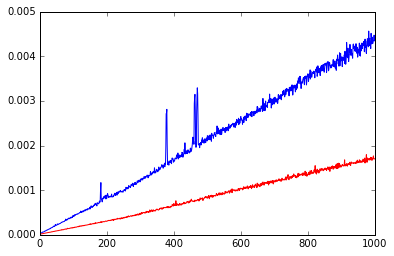
\includegraphics[scale=0.8]{./QuickSort/{pic/q7.png}}
    %\caption{}
\end{figure}
